\section{ \textbf{ساختارها}}

\hspace{13mm} ساختارها شامل \lr{struct} ها، ماکروها، ثابت‌ها و جنس‌های تعریف شده است.

\subsection{\lr{sph-skein-big-context}}
\label{subsec:sph-skein-big-context}
این ساختار مورد نظر برای ذخیره و استفاده از هش است (‌ شامل مقادیری از هش قبلی و مقادیر جدید محاسبه شده ). \\ این ساختار شامل یک آرایه‌ی ۶۴ بیتی از کاراکترها  و   هشت عدد ۶۴ بیتی  که برای ذخیره‌ی ۵۱۲ بیت هش  استفاده می‌شوند  و هم‌چنین شامل دو عدد با نام‌های \lr{ptr, bcount} است که \lr{ptr} به آخرین خانه‌ی پر شده‌ی بافر از دیتا و \lr{bcount} تعداد مضارب صحیح ۵۱۲ کوچکتر از طول دیتا است.


\subsection{\lr{IV512}}
\label{subsec:IV512}
این ساختار شامل مقادیر اولیه‌ی هش است. یک عدد ۵۱۲ بیتی را برای خوانا بودن در مبنای ۱۶ و در ۸ بلاک ۱۶ رقمی نگاه می‌دارد.
\subsection{\lr{UBI-BIG}}
\label{subsec:UBI-BIG}

در این تابع روی دیتای ذخیره شده در بافر، عملیات درهم‌سازی انجام شده‌است. این درهم‌سازی برمبنای مقادیر قبلی موجود در $  h_0 $ تا  $ h_7 $ ( که در سری قبلی صدا شدن این تابع مشخص شده‌اند)، دیتا و ورودی‌های \lr{extra} و  \lr{etype} انجام شده‌است.
در ابتدا سه\lr{ sph-u64 }با اسامی $ t_0 , t_1 , t_2 $ تعریف شده‌اند. \lr{ sph-u64 }جنسی تعریف شده برای متغیرهای ۶۴ بیتی بدون علامت است. با شروع از \lr{buf} هر هشت عنصر که هر کدام یک بایت هستند توسط دیکودر در \lr{sph-dec64le-aligned} به ۶۴ بیت پشت سر هم تبدیل شده و سپس به$ m_0 $تا $ m_7 $ داده شده‌اند. مقدارهای $ m_0 $ تا $ m_7 $ در $ p_0 $ تا $ p_7 $ ریخته شده‌اند. $ m_0 $ تا $ m_7 $ تا اخر تابع بدون تغییر باقی مانده و مقدارهای اولیه‌ی بخش‌های دیتا هستند.
سپس مقدار ‌\lr{extra} پس از \lr{cast} به\lr{sph-u64} با مقدار \lr{bcount} با ۶ بیت شیفت به چپ جمع شده و به $ t_0 $ داده شده‌است. سپس مقدار ‌\lr{bcount} ، ۵۸ بیت به راست شیفت داده شده و ‌\lr{etype} هم ۵۵ بیت به چپ شیفت داده شده‌است. این مقادیر با هم جمع شده‌‌اند و جمعشان به ‌$ t_1 $ داده شده‌است. مقدار شیفت داده شدن‌ها از روی شکل زیر قابل توجیه‌اند:
\begin{center}
	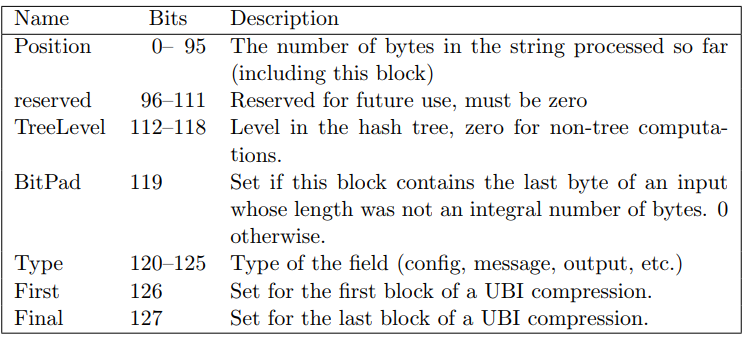
\includegraphics[width=14cm]{images/GoldenModelDocumentation/tweak.png}
\end{center}

در این جدول \lr{TreeLevel} همان \lr{bcount} است که در تابع\hyperref[subsec:skein-big-core]{\lr{skein-big-core}} در هربار صدا کردن \lr{UBI-BIG} مقدار آن یک واحد افزوده می‌شود. \lr{etype} برای رد کردن بخش \lr{position} و هم‌چنین مشخص کردن بیت \lr{first}  است و \lr{extra} برای تعیین بیت \lr{final} و \lr{bitpad} استفاده شده‌است. پنج بیت خالی هم برای \lr{Type}قرار داده شده و هم‌چنین بخش \lr{reserved} هم صفر است.
\\
سپس تابع\hyperref[subsec:TFBIG-KINIT]{\lr{TFBIG-KINIT}}
صدا شده تا مقادیر $ t_2 $ و $ h_8 $ برمبنای بقیه ورودی های تابع یعنی $ t_1 , t_0 $ و $ h_0 $ تا $ h_7 $ تعیین شوند. سپس برای اعداد زوج بین ۰ تا ۱۷\hyperref[subsec:TFBIG-4e]{\lr{TFBIG-4e}} و برای فردها \hyperref[subsec:TFBIG-4o]{\lr{TFBIG-4o}} صدا شده‌است. به این ترتیب میکس در ۱۸ سری چهار تایی اجرا شده که هر کدام ۴ \lr{round} دارند و هر ۸ سری صدا شدن مشابه است و در هر یک از این ۱۸ سری دانستن زوج و فرد بودن سری کافیست. هم‌چنین هر چهار بار یعنی در ابتدای هر \lr{TFBIG-4e}یا\lr{TFBIG-4o} یک بار\hyperref[subsec:TFBIG-ADDKEY]{\lr{TFBIG-ADDKEY}}صدا شده تا بر مبنای شماره‌ی سری که در این‌جا با $ s$ نمایش داده شده و همین‌طور $ i $در $ pi $ و باقی مانده گرفتن از جمعشان کلید جدید مشخص شده و با$ pi $ جمع شود. این‌جا از$ h_0 $تا$ h_7 $که حاصل سری قبلی اجرای\lr{UBI-BIG} است و همین‌طور \lr{tweak} ها استفاده شده تا مقدار جدید $ pi $ تعیین و در سری بعد استفاده شود. سپس برای بار هجدهم \lr{TFBIG-ADDKEY} صدا شده‌است. در نهایت $ hi $ از $ xor $ گرفتن $pi $ و $ mi $ به دست ‌آمده‌است، پس ‌‌‌$ hi $ نشان‌دهنده‌ی بیت‌های تغییر یافته‌ی ‌$ pi $ در طول تابع است.


\subsection{\lr{TFBIG-4e}و \lr{TFBIG-4o}}
\label{subsec:TFBIG-4e}
\label{subsec:TFBIG-4o}

این توابع برای تغییر مقادیر $ p_0 $ تا $ p_7 $ طراحی شده‌است. همان‌طور که پیش‌تر توضیح داده شد، ۷۲ بار تابع درهم‌سازی صدا شده‌،‌ و هر ۸ سلسله از این ۷۲ مرحله یکسان است، هم‌چنین در انتهای هر ۴ مرحله مقدار کلید تغییر   داده شده‌است.
\\
این تابع یک ورودی  \lr{s} دارد. تابع  \hyperref[subsec:TFBIG-ADDKEY]{\lr{TFBIG-ADDKEY }} با ‌$ p_0 $ تا  $ p_7 $ و $ h $ و $ t $و ‌$ s $ به ترتیب به عنوان  $ w_0 $ تا $ w_7 $و $ k $و ‌$ t $ و ‌$ s $ صدا شده‌است. ‌$ h $ و $ t $ برای \lr{concat} و ساختن کلید در تابع \lr{TFBIG-ADDKEY} استفاده شده‌اند. \\
سپس   \hyperref[subsec:TFBIG-MIX8]{\lr{TFBIG-MIX8 }}چهار بار برای ترتیب‌های متفاوتی از ‌$ p_0 $ تا $ p_7 $ با اعداد متفاوت به عنوان $ rc $ صدا شده‌است. ترتیب صدا شدن $ p_0 $ تا $ p_7 $ برای تعداد بلاک ۸ به صورت جدول‌های زیر است،‌ که برای هر ‌‌راند از ۰ تا ۳، بر حسب راند قبل ترتیب‌ها چهار عدد جابه‌جا شده‌اند، و تفاوت حالت‌های زوج و فرد، در اعدادِ استفاده شده است. در جدول‌ها$  N_w$  تعداد \lr{cipher block}هاست که در این کد ۸ است. همین‌طور \lr{j} همان شماره‌‌ی راند در ماژول‌های وریلاگ است.
\begin{center}
	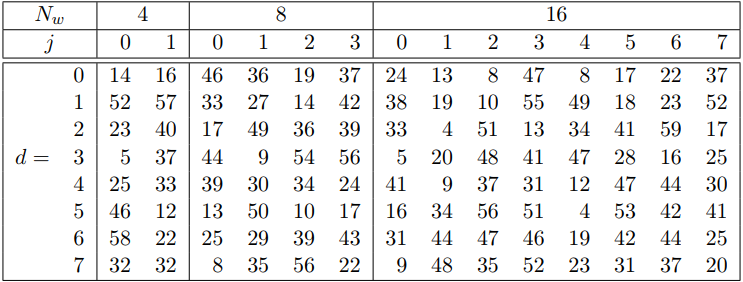
\includegraphics[width=10cm]{images/GoldenModelDocumentation/table_mix.png}
	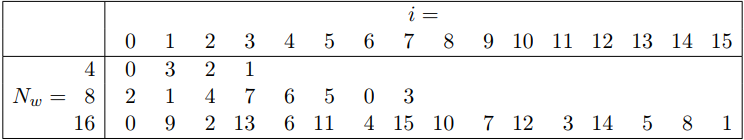
\includegraphics[width= 10cm]{images/GoldenModelDocumentation/Mix2.png}
\end{center}


\subsection{\lr{TFBIG-ADDKEY}}
\label{subsec:TFBIG-ADDKEY}

در این تابع طبق فرمول‌های زیر مقادیر ورودی تغییر داده شده‌است و برای اینکار از تابع‌های \hyperref[subsec:SKBI]{\lr{SKBI}} و \hyperref[subsec:SKBT]{\lr{SKBT}} استفاده شده‌است .
\\متغیرهای $ h_0 $ تا $ h_8 $ در تولید کلید استفاده می‌شوند، برای محاسبه‌ی اندیس آن‌ها ( از ۰ تا ۸ ) از \lr{SKBI} استفاده شده است.
\\
متغیر‌های دیگری که در تولید کلید استفاده شده‌اند $ t_0 $ تا $ t_2 $ هستند که برای تولید اندیس آن‌ها از تابع \lr{SKBT} استفاده شده است.\\
\begin{latin}
	\begin{center}
		\begin{tabular}{l l}
			$k_{s, i} = k_{(s+i) \mod 9} $ \hspace{15mm} & $  i = 0, 1, 2, ... , 4 $ \\
			$k_{s, 5} = k_{(s+5) \mod 9} + t_{s \mod 3}$ & \\
			$k_{s, 6} = k_{(s+6) \mod 9} + t_{(s+1) \mod 3}$ & \\
			$k_{s, 7} = k_{(s+7) \mod 9} + s $ & \\

		\end{tabular}
		\\

	\end{center}
\end{latin}

دقت شود که تمامی این محاسبات برای نوع ۵۱۲ بیتی الگوریتم است.




\subsection{\lr{SKBI}}
\label{subsec:SKBI}

تابع \lr{SKBI} برای محاسبه‌ی اندیس کلید استفاده‌ شده‌است. \\
در الگوریتم برای تولید $k_0 $ تا $ k_8 $ از این ماکرو استفاده شده ‌است. $ k $ و $ s $ و $ i $ به این ماکرو داده ‌شده‌ و سپس $ k $ به \lr{ M9-s-i }متصل می‌شود . \lr{ M9-s-i } باقی‌مانده‌ی ‌$s + i $ بر ۹ تعریف شده‌است.


\subsection{\lr{SKBT}}
\label{subsec:SKBT}
برای تولید $ t_0 $ تا $ t_2 $ از این ماکرو استفاده شده است، $ t $ و $ s $ و ‌$ i $ به این ماکرو داده شده و سپس $ t $ به \lr{M3-s-i} متصل شده است. \lr{M3-s-i}  باقی‌مانده‌ی $ s + i $ بر ۳ تعریف شده است.

\subsection{\lr{TFBIG-MIX8}}
\label{subsec:TFBIG-MIX8}


همان‌طور که در مقدمه گفته‌ شده‌است،‌ هر سری از هشت سری، چهار \lr{round} دارد، پس طراحی این تابع برای ساده‌سازی استفاده‌ی متداول از \hyperref[subsec:TFBIG-MIX]{\lr{TFBIG-MIX}} ‌است. به صورت متداول در کد به چهار سری استفاده از  \lr{TFBIG-MIX} به‌صورت پشت‌ سر هم نیاز است.


\subsection{\lr{TFBIG-MIX}}
\label{subsec:TFBIG-MIX}

وظیفه‌ی این تابع، درهم سازی بلاک‌های ورودی طبق فرمول‌های زیر است.
\begin{center}
	$y_0 = (x_0 + x_1) \mod 2^{64}$ \\
	$ y_1 = (x_1 <<< R_{(d \mod 8), j}) \oplus y_0$
\end{center}
که مقادیر $ R $ در جدول زیر آمده است :

\begin{center}
	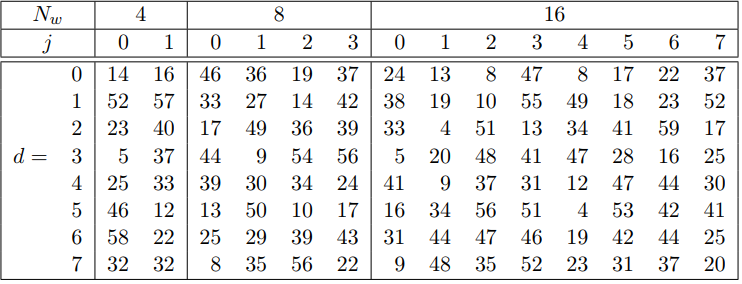
\includegraphics[width=10cm]{images/GoldenModelDocumentation/MIX1.png}
\end{center}




\subsection{\lr{TFBIG-KINIT}}
\label{subsec:TFBIG-KINIT}
در این تابع با ورودی‌های $ t_0 $ تا $ t_2 $ و $h_0 $ تا $ h_8 $ مقادیر زیر محاسبه شده‌است:
$$
k_8 = C \oplus k_0 \oplus k_1 \oplus ... \oplus k_7
$$

$$
t_2 = t_1 \oplus t_0
$$
که مقدار ثابت $ C $ به آن جهت در فرمول وجود دارد که از ۰ نبودن تمامی بیت‌ها اطمینان حاصل شود.

\subsection{\lr{DECL-STATE-BIG}}
\label{subsec:DECL-STATE-BIG}


در این ماکرو متغیرهای ‌$ h_0 $ تا $ h_7 $ و \lr{bcount} از جنس\lr{sph-u64} (متغیر ۶۴بیتی بدون علامت) تعریف شده‌اند.


\subsection{\lr{READ-STATE-BIG}}
\label{subsec:READ-STATE-BIG}


این تابع برای خواندن اطلاعات از ورودی و ذخیره‌ی ‌‌آن‌ها بر روی متغیرهاست. به طور دقیق‌تر  به این تابع ‌بلاک \lr{sc} به عنوان ورودی داده شده‌است. در آن، متغیرهای $ h_0 $ تا $ h_7 $ و \lr{bcount} استراکت به ترتیب به متغیرهای ‌$ h_0 $ تا $ h_7 $ و \lr{bcount} کد مقداردهی شده‌اند.

\subsection{\lr{WRITE-STATE-BIG}}
\label{subsec:WRITE-STATE-BIG}


این تابع برای ذخیره‌ی اطلاعات بر روی \lr{struct} است.\\
به این تابع ورودی \lr{struct}  با نام \lr{sc} داده شده‌است. متغیرهای $ h_0 $ تا $ h_7 $ و همین‌طور \lr{bcount} کد، در $ h_0 $  تا  $ h_ 7 $ و \lr{bcount}  ساختار
ذخیره شده‌اند.

\section{ توابع}

\subsection{\lr{sph-skein512-init}}
\label{subsec:sph-skein512-init}
این تابع مسئولیت مقداردهی اولیه‌ی ساختار هش را بر عهده دارد، که برای آن تابع \hyperref[subsec:skein-big-init]{\lr{skein-big-init}} را با ورودی‌ اولیه‌ی \lr{IV512} اجرا می‌کند.
\subsection{\lr{skein-big-init}}
\label{subsec:skein-big-init}

این تابع دو ورودی می‌پذیرد که یکی از آن‌ها آدرس یک ساختار هش است و دیگری مقدار اولیه است. در این تابع مقادیر متناظر ساختار داده شده برابر مقادیر اولیه قرار گرفته‌اند.
که مقادیر اولیه در حالت ۵۱۲ بیتی در ساختار \lr{IV512} ذخیره شده ‌است.

\subsection{\lr{sph-skein512}}
\label{subsec:sph-skein512}

در این تابع، ماکروی\hyperref[subsec:skein-big-core]{\lr{skein-big-core}} صدا شده‌است. ورودی‌های این تابع که بدون انجام هیچ پردازشی به \hyperref[subsec:skein-big-core]{\lr{skein-big-core}} پاس داده‌ شده‌اند،‌ ‌\lr{cc} که همان ساختار هش است، \lr{data} که داده‌ی ورودی است و ‌\lr{len} که طول  \lr{data} است، هستند.


\subsection{\lr{skein-big-core}}
\label{subsec:skein-big-core}

در این تابع  همه‌ی بلاک‌های دیتا به‌جز بلاک اخر در دسته‌های ۵۱۲ تایی هش شده‌اند. مقدار ‌\lr{bcount} هم برای استفاده‌ی ثانویه تعیین شده و هم‌چنین آخرین بلاک دیتا در بافر ریخته‌ شده‌است. \\به این تابع ورودی‌های ‌\lr{sc} که  ساختار هش است، \lr{data} که داده‌ی ورودی برای هش است و \lr{len} که طول \lr{data} است پاس داده شده‌اند. در ابتدای تابع با صدا شدن \hyperref[subsec:DECL-STATE-BIG]{\lr{DECL-STATE-BIG}} متغیرهای لازم تعریف شده‌اند. سپس در یک $ if $ بررسی شده‌است که برای دیتا در بافر فضای کافی هست یا خیر: \\
- در صورتی که فضا باشد،‌ کل دیتا از جایی که پوینتر به آن اشاره کرده‌است دخیره شده‌ و سپس پوینتر که به پایان دیتای ذخیره شده اشاره دارد، به اندازه‌ی طول دیتا به جلو جابه‌جا شده‌است. در خود ‌\lr{struct} هم مقدار ‌آن \lr{update} شده‌ و سپس از تابع خارج شده‌است.
\\
- در غیر این صورت، ابتدا  \hyperref[subsec:READ-STATE-BIG]{\lr{READ-STATE-BIG}} صدا شده‌است. متغیر \lr{first} یک متغیر هشت بیتی با  مقدار ۰ یا ۱۲۸ است. اگر این تابع به طور متدوال از \hyperref[subsec:skein-hash]{\lr{skein-hash}} صدا شود \lr{first} برابر با ۱۲۸ می‌شود. سپس در یک لوپ ابتدا در صورت پر بودن بافر از دیتا (به این معنی که پوینتر برابر با سایز بافر شده‌باشد)،‌ اول  \lr{bcount} یکی زیاد شده، سپس\hyperref[subsec:UBI-BIG]{\lr{UBI-BIG}} با ورودی‌های $ first + 96 $ به عنوان \lr{etype} و ۰ به عنوان \lr{extra} صدا شده‌است. پس از آن \lr{first} و \lr{ptr} هر دو صفر گذاشته شده‌اند تا برای سری بعدِ پر شدن دیتا، بافر از ابتدا \lr{overwrite} شود. سپس شرط پر بودن بافر تمام شده و به اندازه‌ی مینیموم مقداری که در بافر جا هست با طول دیتای باقی‌مانده، دیتا در بافر ذخیره شده‌است. پوینتر و دیتا با مقدار این مینیموم جمع و \lr{len} منهای آن شده‌ تا مقدار دیتای باقی‌مانده را نشان دهد. سپس حلقه تا زمانی که هنوز دیتایی باقی مانده‌باشد تکرار می‌شود. درواقع در این حلقه هر سری به تعداد بزرگترین مضرب سایز بافر که اکیدا کوچک‌تر از \lr{len} دیتا است تکرار شده و هر سری روی همان طول از دیتا \hyperref[subsec:UBI-BIG]{\lr{UBI-BIG}} صدا شده‌است. \lr{bcount} همین تعداد بار را نشان می‌دهد. آخرین بلاک دیتا که کوچک‌تر مساوی سایز بافر است، در بافر ذخیره شده و \lr{ptr} به آخر آن اشاره کرده‌است.
در آخر \hyperref[subsec:WRITE-STATE-BIG]{\lr{WRITE-STATE-BIG}}
صدا و بعد مقدار فعلی پوینتر هم در \lr{struct} ذخیره شده‌است.
نحوه ذخیره‌سازی \lr{tweak} به شکل زیر است.
\begin{center}
	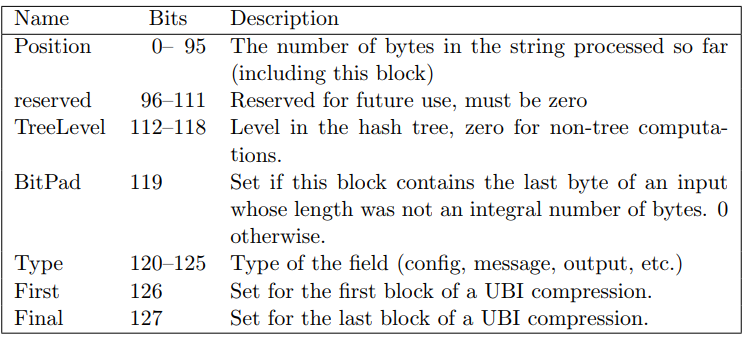
\includegraphics[width=14cm]{images/GoldenModelDocumentation/tweak.png}
\end{center}

دلیل جمع کردن \lr{first} با ۹۶،‌ رد کردن بخش \lr{position} است. حالت اولیه \lr{first} هم به این علت با چک کردن \lr{bcount} مقداردهی شده که مقدار بخش \lr{first} باید برای سری اول گرفتن بلوک دیتا برابر با ۱ باشد.

در این تابع ممکن است سایز دیتا دقیقا مضربی از سایز بلاک (۵۱۲) باشد،‌ برای این حالت باید مقدار بیت \lr{final} یک شود، اما این تابع از این که در حال پردازش اخرین بخش دیتا هست یا نه باخبر نیست و درنتیجه در‌ آخر ممکن است بافر شامل یک بلاک کامل از دیتا باشد.



\subsection{\lr{skein-hash}}
\label{subsec:skein-hash}
\\



در این تابع ابتدا هش از جنس آرایه‌ای ۶۴ تایی از کاراکتر‌های بدون علامت (\lr{uint8-t}) و سپس متغیری با نام \lr{ctx}، ساختاری از جنس  
 \hyperref[subsec:sph-skein-big-context]{\lr{sph-skein-big-context}} 
 تعریف شده‌است. این هش ۵۱۲ در ۵۱۲ است و به همین دلیل حاصل نهایی هم ۶۴ بایت درنظر گرفته شده است. سپس آدرس \lr{ctx} به تابع\hyperref[subsec:sph-skein512-init]{\lr{sph-skein512-init}} پاس داده شده‌است. در این تابع مقدارهای اولیه در ‌\lr{struct} ذخیره شده‌اند. سپس تابع \hyperref[subsec:sph-skein512]{\lr{sph-skein512}} صدا شده که در آن تمام بلاک‌های دیتا به جز بلاک آخر هش شده و بلاک ‌اخر هم در بافر ذخیره شده‌است. سپس تابع  \hyperref[subsec:sph-skein512-close]{\lr{sph-skein512-close}} صدا شده و به آن ‌\lr{struct} و ادرس شروع \lr{hash} داده شده‌اند. در این مرحله بیت‌های اضافی اضافه شده‌اند. بلاک ‌آخر هش شده و در ‌\lr{dst} ذخیره شده‌است.
در نهایت ۳۲ بایت از \lr{hash} در \lr{output} ریخته شده‌است.


\subsection{\lr{sph-skein512-close}}
\label{subsec:sph-skein512-close}
\label{subsec:sph-close}
در این تابع   \hyperref[subsec:addbits]{\lr{sph-skein-addbits-and-close}}  صدا شده و به ‌آن  ساختار  \lr{cc} ،  ادرس  \lr{dst} و همین طور صفر به عنوان \lr{ub} که بیت‌های اضافه است و \lr{n} که تعداد این بیت‌های اضافه است داده شده‌اند.


\subsection{\lr{sph-skein-addbits-and-close}}
\label{subsec:addbits}
\label{subsec:sph-skein-addbits-and-close}
در این تابع  \hyperref[subsec:big-close]{\lr{skein-big-close}} با مقدار ۶۴ برای \lr{out-len} و \hyperref[subsec:sph-skein512-init]{\lr{sph-skein512-init}} صدا شده‌اند. کار درهم‌سازی در \lr{skein-big-close} تمام و سپس دوباره $ h_0 $ تا $ h_7 $ از مقدارهای اولیه پر شده‌اند.


\subsection{\lr{skein-big-close}}
\label{subsec:big-close}
به این تابع ورودی‌های  \lr{sc} به عنوان ساختار هش،  \lr{ub} به عنوان بیت‌های اضافه، \lr{n} به عنوان تعداد بیت‌های اضافه،  \lr{dst} برای ذخیره هش نهایی و  \lr{out-len} به عنوان طول دیتا پاس داده شده‌اند. با توجه به هشت بیتی بودن بلوک‌ها در حداکثر مقدار ‌\lr{n}  هشت است. در نتیجه در صورت غیر صفر بودن ‌\lr{n} ،با شیفت دادن ۱۲۸ به اندازه‌ی  \lr{n}،  متغیری به نام   \lr{z} با  \lr{n} بیت صفر در سمت راست و سپس یک بیت ۱ ساخته‌ شده‌است. سپس  با  \lr{and} کردن  \lr{ub} با    \lr{-z}،  \lr{n} بیت سمت راست  \lr{ub} صفر شده و این مقدار به \lr{x} داده شده ‌است. (زیرا  \lr{z} به صورت مکمل دو منفی شده‌است.) سپس بیت  \lr{n+1}م  \lr{ub} با \lr{or} گرفته‌شدن با \lr{z} ، ۱ شده‌است. سپس  \hyperref[subsec:skein-big-core]{\lr{skein-big-core}} برای طول ۱ صدا شده‌است. (زیرا طول ‌\lr{x} یک بایت است.)  شرط بررسی   \lr{n} اینجا به پایان رسیده‌است.
سپس \hyperref[subsec:read-state-big]{\lr{read-state-big}} صدا و بعد از ‌آن باقی‌مانده‌ی فضای بافر با ۰ پر شده‌است.
سپس دو دفعه  \hyperref[subsec:ubi-big]{\lr{UBI-BIG}} صدا شده‌است. در دفعه‌ی اول صدا شدن تابع،  \lr{etype} برابر جمع (256 + 96) با ۱۲۸ ،در صورت ۰ بودن  \lr{bcount} است و ۹۶ + ۱۲۸ در صورت غیر صفر بودن آن.  همین‌طور در صورت غیر صفر بودن ‌ \lr{n} عدد یک هم با  \lr{etype} جمع شده‌است.  \lr{extra} هم برابر با مقدار \lr{ptr} گذاشته شده‌است،‌ که در زمان صدا کردن تابع به اخرین جایی که دیتا در بافر هست و بیت‌های بعدی ‌آن با ۰ پر شده‌اند، اشاره دارد. جمع شدن ۲۵۶ با  \lr{etype} برای یک گذاشتن  \lr{BitPad} و جمع شدن ۹۶ برای اسکیپ کردن بخش  \lr{position} است. پیش از صدا شدن تابع برای بار دوم کل بافر با ۰ پر و  \lr{bcount} هم برابر با ۰ گذاشته شده‌است. بار دوم  \lr{UBI-BIG} برای  \lr{etype} با مقدار ۵۱۲ و \lr{extra} با مقدار ۸ صدا شده‌است. در ۵۱۰ فقط بیت دوم از راست یک است، که بیت \lr{final} است و ۸ بایت بافر با ۰ پر شده‌است. درنتیجه \lr{extra} هم ۸ است.
در نهایت $ h_0 $ تا $ h_7 $ توسط \lr{sph-enc64le-aligned} بایت بایت شده و در بافر ذخیره شده‌است، و سپس بافر به تعداد بایت \lr{out-len} (در این‌جا ۶۴ بایت) در \lr{dst} ذخیره شده‌است.